\chapter{Design and Implementation}
\label{ch:design_implementation}
This chapter describes the design and implementation of the delegation mechanisms integrated into vodle, detailing both the technical approach and practical decisions made throughout development. It begins by outlining vodle's existing system architecture, clarifying how this influenced the integration of new delegation features. 

Each subsequent section aligns directly with one of the project objectives defined previously, explaining the rationale behind key design choices, algorithms, and interface elements. Emphasis is placed on the critical design trade-offs and challenges encountered, highlighting how constraints such as the serverless architecture and client-side computation informed implementation decisions.

\section{System Architecture Overview}\label{sec:design_architecture}
Vodle is built as a serverless web application that emphasises accessibility, client-side performance, and ease of deployment. Its architecture comprises two components:

\begin{enumerate}
  \item \textbf{Frontend:} Implemented using Angular and the Ionic framework, the frontend provides a responsive and modular interface that works across both desktop and mobile devices. The use of Angular facilitates the creation of component-based user interfaces, essential for introducing interactive features such as the ranked delegation UI and weighted delegation sliders.
  \item \textbf{Backend:} Vodle uses CouchDB as its database. There is no custom backend logic or middleware; instead, the frontend application communicates directly with CouchDB over HTTP.
\end{enumerate}

\subsubsection{Implications of This Architecture}
Vodle's serverless architecture has several implications for the design and implementation of the delegation mechanisms, especially due to the absence of a traditional data processing backend. The following points summarise the key considerations:
\begin{itemize}
  \item All vote delegation logic, including transitive resolution, cycle detection, and weighted delegation calculations, must be executed in the browser. This places constraints on performance and requires careful optimisation of algorithms used.
  \item CouchDB's document-based storage model means that all data must be serialised and deserialised in JSON format. This affects how data structures are designed and manipulated, as well as how they are stored and retrieved from the database.
\end{itemize}

\subsection{CouchDB Storage and Write Constraints}
\label{subsec:couchdb_limits}

Vodle store all data in CouchDB in two types of databases: the \_users database and poll databases. The \_users database is a standard CouchDB database that stores user documents, while the poll databases are created dynamically for each poll and contain all relevant data for that poll.

\begin{enumerate}
  \item \textbf{\_users Database.}
    \begin{itemize}
      \item Each document ID is \texttt{org.couchdb.user:<username>}.
      \item Only the account owner or an administrator may modify or delete their user document.
    \end{itemize}

  \item \textbf{Poll Databases.}
    \begin{itemize}
      \item Databases are named \texttt{poll-<POLLID>}.
      \item Stores:
        \begin{itemize}
          \item The immutable poll definition (\texttt{poll.json}).
          \item One vote document per voter (\texttt{vote-<user>}).
        \end{itemize}
    \end{itemize}
\end{enumerate}

\paragraph{Document-Level Security}
CouchDB enforces security at the level of entire documents. This means that access control decisions are made based on the identity of the user attempting to write a document and the document's ID -- there is no support for restricting access to individual fields within a document. Additionally, CouchDB does not support merging concurrent changes; updates must replace the entire document in a single write operation. As a result, all write operations are either fully accepted or fully rejected by the database's \texttt{validate\_doc\_update} function. This strict model simplifies validation logic but introduces important constraints in the context of implemented liquid democracy, which are discussed in the remainder of this section.

\subsubsection{Poll-DB Validation}
When a client writes to a poll database, the \texttt{validate\_doc\_update} enforces:

\begin{enumerate}
  \item \textbf{User Documents:} IDs are prefixed with \texttt{~vodle.user.}, and only the owner may modify them:
\begin{figure}[H]
  \centering
\begin{minted}{typescript}
if (!id.startsWith(`~{userCtx.name}§`)) {
  throw({ forbidden: 'Only the document owner may modify this user doc.' });
}
\end{minted}
\caption{Code to prevent a user from modifying another user's document.}
\end{figure}

  \item \textbf{Immutable Poll Artefacts: } Documents like \texttt{poll.json} or results cannot be updated once created:
\begin{figure}[H]
    \begin{minted}[fontsize=\small,baselinestretch=1]{javascript}
if (oldDoc && isPollArtifact(id)) {
  throw({ forbidden: 'Poll documents are immutable once created.' });
}
    \end{minted}
\caption{Code to prevent modification of poll artefacts.}
\end{figure}
\end{enumerate}

\subsubsection{\_users-DB Validation}
In the \_users database, a similar validation function is used to prevent users from modifying other users' documents, including the \texttt{vodle} service account.
\begin{figure}[H]
\begin{minted}[fontsize=\small,baselinestretch=1]{javascript}
if (id !== `org.couchdb.user:{userCtx.name}`) {
  throw({ forbidden: 'Users may only modify their own user document.' });
}
if (userCtx.name === 'vodle' || isPollService(userCtx.name)) {
  throw({ forbidden: 'Service accounts are immutable.' });
}
\end{minted}
\caption{Code to prevent a user from modifying another user's document.}
\end{figure}

\subsection{Summary of Storage and Validation Constraints}
\label{subsec:summary_storage_constraints}

The architecture of vodle, particularly its reliance on CouchDB and the absence of a custom backend, imposes important constraints on how delegation features are designed and implemented.

\begin{itemize}
  \item \textbf{User autonomy is strictly enforced.} Each user can only modify documents that are explicitly associated with their own identity. This guarantees that vote and delegation data cannot be tampered with by other clients but also eliminates the possibility of directly setting or managing another user's vote.

  \item \textbf{Issues with sharing a document.} The current database design does not support the modification of a single document by multiple users. As a result, features that require a global view -- such as a delegation graph -- require a rework of the database schema.

  \item \textbf{Validation logic is structural, not contextual.} Since CouchDB validation functions can only inspect the document being written, they cannot reason about relationships across documents. This prohibits logic such as resolving delegations server-side, enforcing uniqueness of votes, or validating delegation cycles at the point of write.

  \item \textbf{Client-side logic carries the burden.} Due to previous point, all logic for delegation resolution, cycle checking, and weighted delegation must be implemented in the client. This requires careful design to ensure that the frontend can handle complex delegation scenarios without overwhelming the user or causing performance issues.
\end{itemize}

Together, these constraints shape some of the design and implementation choices of the delegation features in vodle, which will be discussed in detail in the following sections.

% \subsection{Existing Implementation of Liquid Democracy}\label{subsec:design_existing_implementation}
% As mentioned in the background research (see Section~\ref{subsec:background_existing_delegation}), vodle already contained a partial implementation of liquid democracy prior to this project. This early version was not activated in production and was ultimately left incomplete due to stability and design issues. Despite this, it included a basic delegation model that served as a foundation for completing objective 1.

% The following subsection outline the key features of the original implementation, including its strengths and issues, which were addressed in the redesigned system.
% % However, the underlying logic was incomplete and unreliable. Delegation data was handled entirely on the client side, and there was no mechanism for synchronising delegation state between users. This led to inconsistencies in features such as cycle detection, which was applied inconsistently depending on the client's local state. Furthermore, no resolution model was implemented for handling transitive delegations or more complex delegation structures.

% % Despite these limitations, several components from the original system were retained during redevelopment. These included parts of the invitation system and select UI elements that handled delegation acceptance and rejection. These elements were adapted and extended as part of the redesigned delegation model, which introduced reliable state management, cycle prevention, and support for advanced delegation behaviours. The subsequent sections detail how this new model was implemented and integrated into vodle.

% \subsubsection{Delegation Interaction Flow}
% The original delegation mechanism in vodle was built around an explicit, opt-in invitation model. Under this model, a user could not be designated as a delegate without their knowledge or consent, thereby preserving both vote privacy and user autonomy. Delegation was initiated by one user (the \textit{delegator}) and required an explicit response (either acceptance or rejection) from the other party (the \textit{delegate}) before it became active.

% Figure~\ref{fig:delegation-flow-accept} illustrates the standard interaction sequence. In step 1, user A generates and shares a unique delegation link with user B. This link encodes A's intent to delegate and provides B with a prompt to either accept or reject the invitation. If B accepts (step 2), A adopts B's vote as their own (shown by a dashed arrow), while B proceeds to cast their vote independently. Crucially, the delegation only becomes effective upon B's confirmation.

% If B instead rejects the invitation (Figure~\ref{fig:delegation-flow-reject}), both users cast their votes independently. In either case, the process is explicit and reversible: B can update their decision at any time, and A can cancel or resend the delegation request as needed.

% This interaction flow has two key strengths. First, it ensured that delegations could not be made unilaterally - a voter could never become a delegate without their knowledge. Second, it provided a simple and intuitive interface for forming delegation links (which could be shared via email, social platforms, or by copying the link), lowering the barrier to entry for new users.

% However, while this implementation excelled at user autonomy and privacy, it lacked critical safeguards such as a consistent mechanism to prevent delegation cycles. The following section discusses the limitations of the original cycle-checking logic and outlines how these issues were addressed in the redesigned system.

% \subsubsection{Cycle Checking}
% Cycle prevention is necessary to ensure that delegated votes always reach a valid casting voter. If a cycle forms -- such as A delegating to B, B to C, and C back to A -- then no vote is cast at the end of that chain, causing all involved votes to be nullified. This can seriously undermine the integrity of the final result.

% The original implementation in vodle attempted to prevent such cycles but applied this logic inconsistently. Cycle detection relied on the local view of the delegation graph cached in each user's browser. Since there was no mechanism for synchronising delegation state between clients, different users could have contradictory views of the system. This meant that a delegation rejected on one device (due to a perceived cycle) might succeed on another. The lack of real-time propagation also led to user interface inconsistencies, where delegation controls displayed outdated or misleading information.

% Internally, the system attempted to detect cycles when a user received a delegation request by checking for existing direct or indirect delegations back to the requester. The code used a combination of local delegation maps, including the \verb|direct_delegation_map| and \verb|effective_delegation_map|, to approximate whether a cycle might form. The logic for determining if a cycle or two-way delegation would occur can be seen in the following code snippet:

% \begin{minted}{typescript}
% const effdel_vid = effdelmap.get(oid).get(myvid) || myvid;
% if ((dirdelmap.get(oid) || new Map()).get(myvid) == client_vid) {
%   two_way = true;
% } else if (effdel_vid == client_vid) {
%   cycle = true;
% }
% \end{minted}

% Here, the code checks if the effective delegate (casting voter) of the responder (\verb|effdel_vid|) is equal to the original requester (\verb|client_vid|). If so, it flags the possibility of a cycle.

% Despite these precautions, the absence of a global, shared delegation graph meant that cycle prevention was never fully reliable. Cycles could still occur due to race conditions or stale client views. This instability, coupled with the challenge of maintaining consistent cycle detection across browsers, was a key reason why delegation features were disabled in production at the time.

% In the redesigned system, these issues are addressed through a shared, synchronised data structure that tracks delegation across all users. This enables consistent validation of new delegations and real-time detection of cycles regardless of which client initiates or accepts a delegation. The design and implementation of this new cycle detection mechanism (as part of completing Objective 1) are described in Section~\ref{subsec:obj1_cycle_checking}.

% \subsubsection{Inconsistent User Interface}

\section{Implement a Core Delegation Model into vodle}\label{sec:core_delegation_detailed}
This section outlines the design and implementation of the core delegation model within vodle, addressing Objective 1 of the project. It begins with an analysis of the pre-existing, partially implemented delegation system, identifying the limitations that motivated a full redesign. The second half of the section describes the final implementation, including the new data structures, algorithms, and interface improvements introduced.

\subsection{Limitations of the Pre-existing Implementation}

Before this project began, vodle included a partially implemented delegation system. Although disabled due to critical flaws, the system introduced several foundational ideas and structures that influenced the final design. This section introduces the key data structures used in the original model, explains the intended delegation flow, and analyses why a full redesign was necessary.

\subsubsection*{Delegation Maps}

The delegation mechanism relied on several maps to track how votes were delegated and resolved. These maps were stored and updated locally on each client:

\begin{itemize}
    \item \textbf{direct\_delegation\_map}: This map recorded direct delegation relationships. For each option ID (\texttt{oid}), it stored a mapping from voter IDs to the user they directly delegated to.

    \item \textbf{effective\_delegation\_map}: This map stored the final casting voter for each user by resolving the full transitive chain of delegations. For example, if user A delegated to B and B delegated to C, the effective delegate of A was C.

    \item \textbf{inv\_effective\_delegation\_map}: The inverse of the effective map. For each user, it stored the set of voters whose votes were ultimately counted under them. This was useful for computing voting weights and for cycle detection.
\end{itemize}

Each map was maintained locally by the browser and not synchronised across clients. This made the correctness of delegation state dependent on each user's local view.

\subsubsection*{Delegation Flow}

Delegation in vodle followed an explicit, link-based invitation model:

\begin{enumerate}
    \item A user (the delegator) generated a delegation ID (DID), created a key pair, and constructed a \texttt{del\_request} object specifying the options to delegate.
    \item A magic link containing this information was shared with the intended delegate.
    \item The delegate could accept or reject the invitation. If accepted, a signed \texttt{del\_response} was created, completing the delegation handshake.
    \item Once accepted, a \texttt{del\_agreement} object was created and cached by both parties. This structure tracked which options were accepted and which were currently active.
\end{enumerate}

This invitation model upheld user autonomy: users could not be delegated to without their explicit consent. Delegation could also be revoked at any time and overridden on a per-option basis.

\begin{figure}[H]
  \centering
  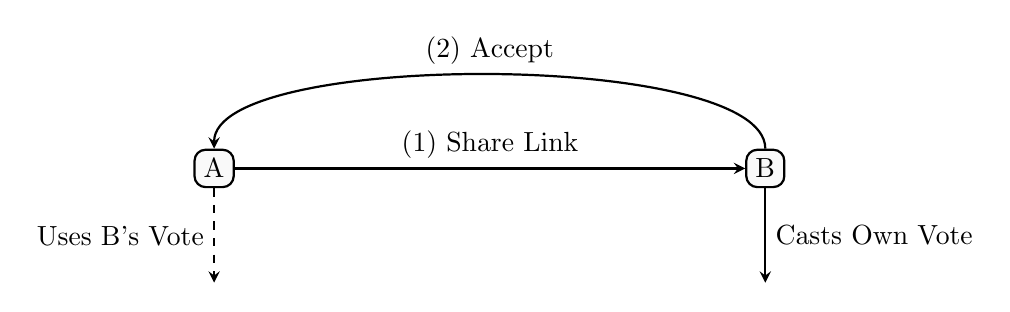
\begin{tikzpicture}[node distance=7cm,>=stealth,thick]
    % clients
    \node[rectangle,draw,rounded corners,fill=gray!5] (A) {A};
    \node[rectangle,draw,rounded corners,fill=gray!5,right of=A] (B) {B};
    % arrows
    \draw[->] (A) -- node[above]{(1) Share Link} (B);
    \draw[->] (B) .. controls +(0,1.5) and +(0,1.5) .. node[above]{(2) Accept} (A);
    \draw[->] (B.south) -- ++(0,-1.2) node[midway,right]{Casts Own Vote};
    \draw[->, dashed] (A.south) -- ++(0,-1.2) node[midway,left]{Uses B's Vote};
  \end{tikzpicture}
  \caption{Sequence for a delegation to be initiated. User A shares a link with user B, who accepts the delegation.}
  \label{fig:delegation-flow-accept}
\end{figure}

\begin{figure}[H]
  \centering
  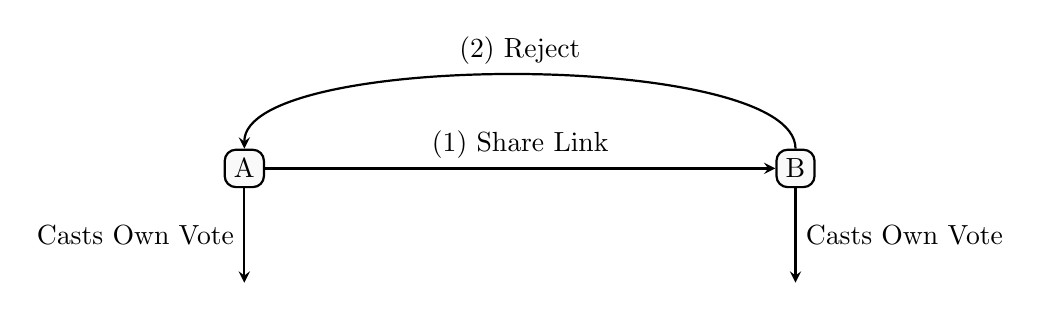
\begin{tikzpicture}[node distance=7cm,>=stealth,thick]
    % clients
    \node[rectangle,draw,rounded corners,fill=gray!5] (A) {A};
    \node[rectangle,draw,rounded corners,fill=gray!5,right of=A] (B) {B};
    % arrows
    \draw[->] (A) -- node[above]{(1) Share Link} (B);
    \draw[->] (B) .. controls +(0,1.5) and +(0,1.5) .. node[above]{(2) Reject} (A);
    \draw[->] (B.south) -- ++(0,-1.2) node[midway,right]{Casts Own Vote};
    \draw[->] (A.south) -- ++(0,-1.2) node[midway,left]{Casts Own Vote};
  \end{tikzpicture}
  \caption{Sequence for a rejected delegation. User A shares a delegation link with user B, who rejects the delegation.}
  \label{fig:delegation-flow-reject}
\end{figure}


\subsubsection*{Cycle Detection Failures}

The main flaw in the system was its inability to reliably prevent delegation cycles. A cycle occurs when a user indirectly delegates back to themselves, such as in the sequence A~$\rightarrow$~B~$\rightarrow$~C~$\rightarrow$~A. In such cases, the vote becomes trapped and is not cast.

Clients attempted to detect cycles during the delegation acceptance phase by examining local delegation maps. A typical check would confirm whether the proposed delegate was already an effective delegate of the user. If so, the client marked the request as cyclic and blocked it.

However, because these maps were not synchronised, different clients could hold conflicting views of the delegation graph. A delegation that passed validation on one device might cause a cycle once accepted, or be silently invalidated by another. This undermined correctness and made vote resolution unpredictable.

\subsubsection*{User Interface Limitations}

\subsubsection*{Summary}

The original delegation system implemented many strong conceptual ideas. It preserved user autonomy through an invitation model, allowed for fine-grained control over delegated options, and supported transitive delegation. However, it relied entirely on client-local data and logic. Without a global, synchronised delegation graph, the system could not reliably detect cycles or ensure consistent resolution of votes. These limitations made it unsuitable for deployment and motivated a full redesign, described in the next section.

\subsection{Revised Implementation}
This section describes the final design and implementation of the core delegation mechanism in vodle, which allows users to delegate their votes to others. It addresses the limitations of the original system by introducing a global, synchronised delegation graph, efficient cycle prevention, and consistent transitive resolution logic. The design preserves the invitation-based flow and per-option control from the earlier implementation while ensuring correctness across all clients.

\subsubsection*{Cycle Checking: Algorithm and Rationale}
We can represent delegation relationships as a directed graph, where users are nodes and delegations form directed edges. A valid vote delegation must not introduce cycles in this graph: for example, a sequence such as A~$\rightarrow$~B~$\rightarrow$~C~$\rightarrow$~A would result in all votes becoming trapped, with no final casting voter. Therefore, delegation cycles must be proactively prevented at the time a new delegation is proposed.

A proposed delegation from user $X$ to user $Y$ is valid if and only if $Y$ is not a descendant of $X$ in the current delegation graph. That is, there must be no existing path from $Y$ back to $X$.

% \subsection*{Delegation Graph and Cycle Checking}\label{subsec:obj1_cycle_checking}
% Delegations are represented as a directed graph, where each user is a node and each delegation is a directed edge from a delegator to their delegate. Preventing cycles in this graph is essential to guarantee that every vote can be correctly resolved to a casting user.

% Rather than recomputing the full graph for each delegation attempt, the algorithm maintains a data structure called the \texttt{inverse\_indirect\_map}, which stores the transitive descendants of each user.

Instead of checking for this condition directly using a depth-first search (DFS) or breadth-first search (BFS), a more efficient approach is to maintain a list of all descendants for each user. This allows us to check if $Y$ is in the list of descendants of $X$ in constant time. The implementation details of this approach is detailed in the next section.

\subsubsection{Implementation Details}
A hashmap is used to store the descendants of each user. The keys are user IDs, and the values are sets of user IDs representing the direct delegates of that user. In the code, this hashmap is referred to as ``\verb|inverse_indirect_map|''.

Suppose the following delegations exist:
\begin{itemize}
    \item A delegates to B
    \item B delegates to C
    \item C delegates to D
\end{itemize}

The resulting \texttt{inverse\_indirect\_map} is:
\begin{figure}[H]
  \centering
  \begin{minted}{python}
    inverse_indirect_map = {
      "B": {"A"},
      "C": {"B", "A"},
      "D": {"C", "B", "A"}
    }
    \end{minted}
  %\caption{Example of a hashmap for users A, B, C, and D. User A has delegated to B, user B has delegated to C, and user C has delegated to D. Consequently, the descendants of user D are A, B and C.}
  \label{fig:inverse_indirect_map}
\end{figure}

This map enables several key operations required for maintaining a consistent and cycle-free delegation graph:

\begin{itemize}
  \item \textbf{Check Delegation Validity:} To determine whether a delegation \(X \!\to\! Y\) would create a cycle, the system checks if \(Y\) already appears in the set of descendants of \(X\). If so, the new delegation is invalid. This check takes \(O(1)\) time.
  \begin{figure}[H]
    \centering
    \begin{minted}{javascript}
      const inverse_indirect_map = this.G.D.get_inverse_indirect_map(pid);
      const descendant_set = inverse_indirect_map.get(delegate_vid);
      if (descendant_set.has(myvid)) {
        cycle = true;
      }
    \end{minted}
    \caption{Code for checking if a delegation is valid. This check is triggered when a user clicks on a delegate link. The map is retrieved from the synchronised local cache, and the set of descendants is used to confirm that a cycle would not be formed.}
  \end{figure}

  \item \textbf{Add Delegation Edge:} When a new delegation \(X \to Y\) is accepted, the system must ensure that the descendant relationship is updated consistently. Specifically, for $Y$ and every user \(u\) such that \(Y \in \texttt{desc}(u)\), their descendants must be updated to include both \(X\) and all of \(X\)'s current descendants.

  \item \textbf{Remove Delegation Edge:} When a delegation \(X \!\to\! Y\) is removed, the system must ensure that the descendant relationship is updated consistently. Specifically, for $Y$ and every user \(u\) such that \(Y \in \texttt{desc}(u)\), their descendants must be updated to remove both \(X\) and all of \(X\)'s current descendants.
\end{itemize}

\subsubsection{User Interface -- TODO: add screenshots and actually fill in}
\begin{itemize}
\item Create delegation invite line
\item Accept screen
\item Accept screen when there is a cycle
\item UI from user A POV (votes are being controlled)
\begin{itemize}
  \item Note Fixes:
  \item controls some-all-none of your votes
  \item your vote is used for n-other delegates
\end{itemize}
\item UI from user B POV (Is a delegate)
\end{itemize}

\begin{figure}[H]
  \centering
  \begin{subfigure}[t]{0.28\linewidth}
    \centering
    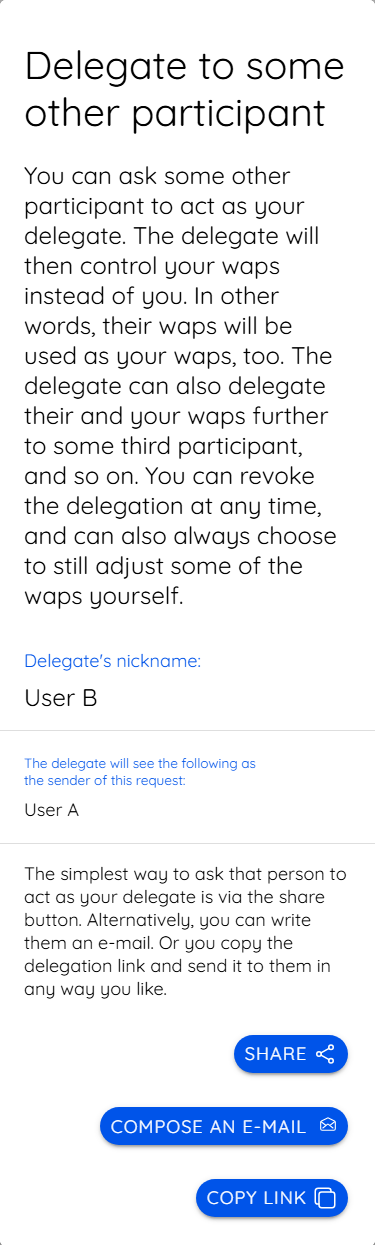
\includegraphics[width=\linewidth]{../common/initial_vodle_screenshots/deldialog.png}
    \caption{User A's invitation screen.}
    \label{fig:del-dialog}
  \end{subfigure}
  \hfill
  \begin{subfigure}[b]{0.68\linewidth}
    \centering
    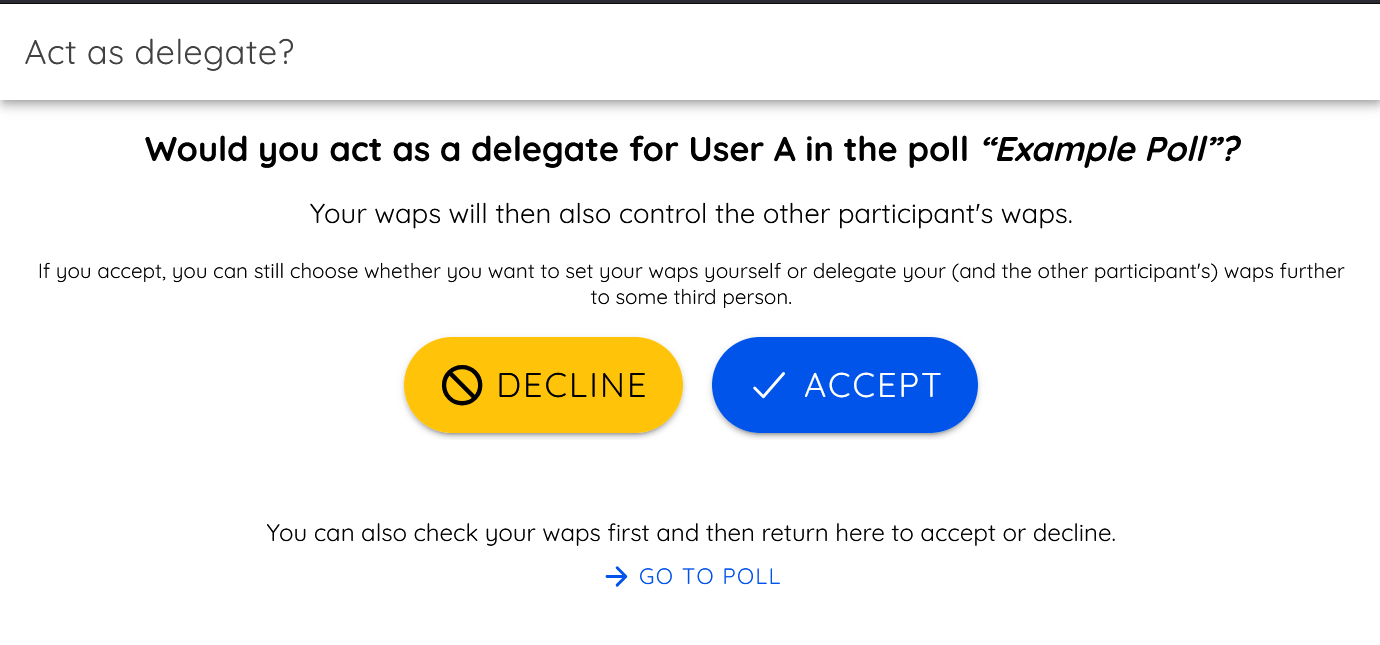
\includegraphics[width=\linewidth]{../common/initial_vodle_screenshots/delaccept.png}
    \caption{User B's delegation acceptance screen when there is no cycle.}
    \label{fig:del-accept}
    
    \vspace{1em}
    
    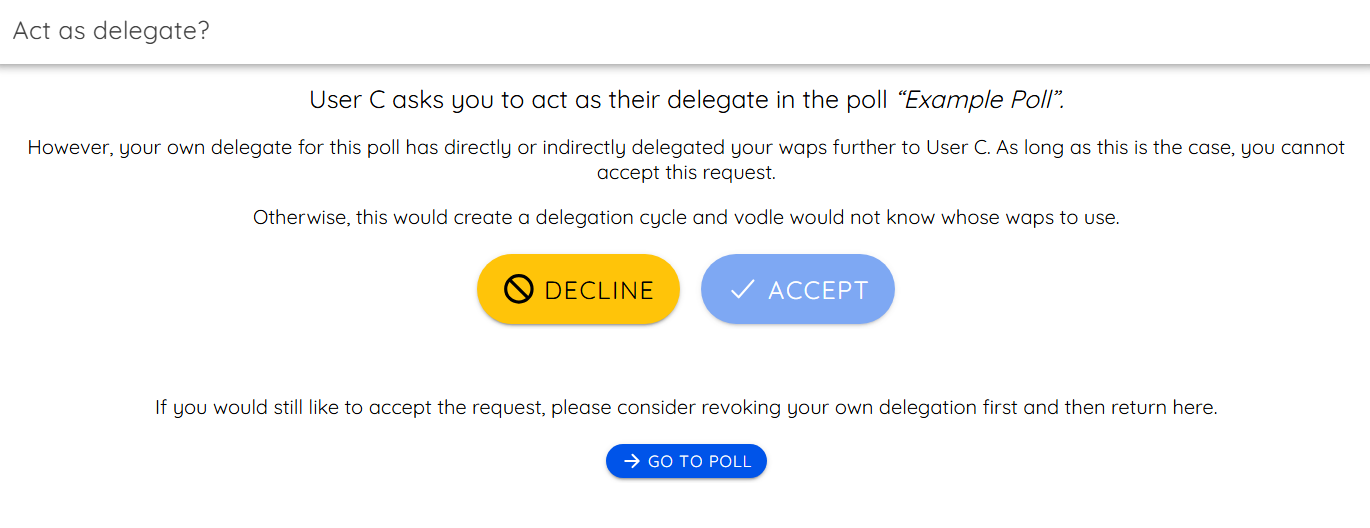
\includegraphics[width=\linewidth]{../common/initial_vodle_screenshots/delaccept_cycle.png}
    \caption{User A's screen after opening a delegation link from User C (who User B has delegated to).}
    \label{fig:del-accept-cycle}
  \end{subfigure}
  \caption{Screens shown to Users A and B during the delegation invitation and response process.}
  \label{fig:delegation-accept-flow}
\end{figure}


\begin{figure}[H]
  \centering
  \begin{subfigure}[t]{0.8\linewidth}
    \centering
    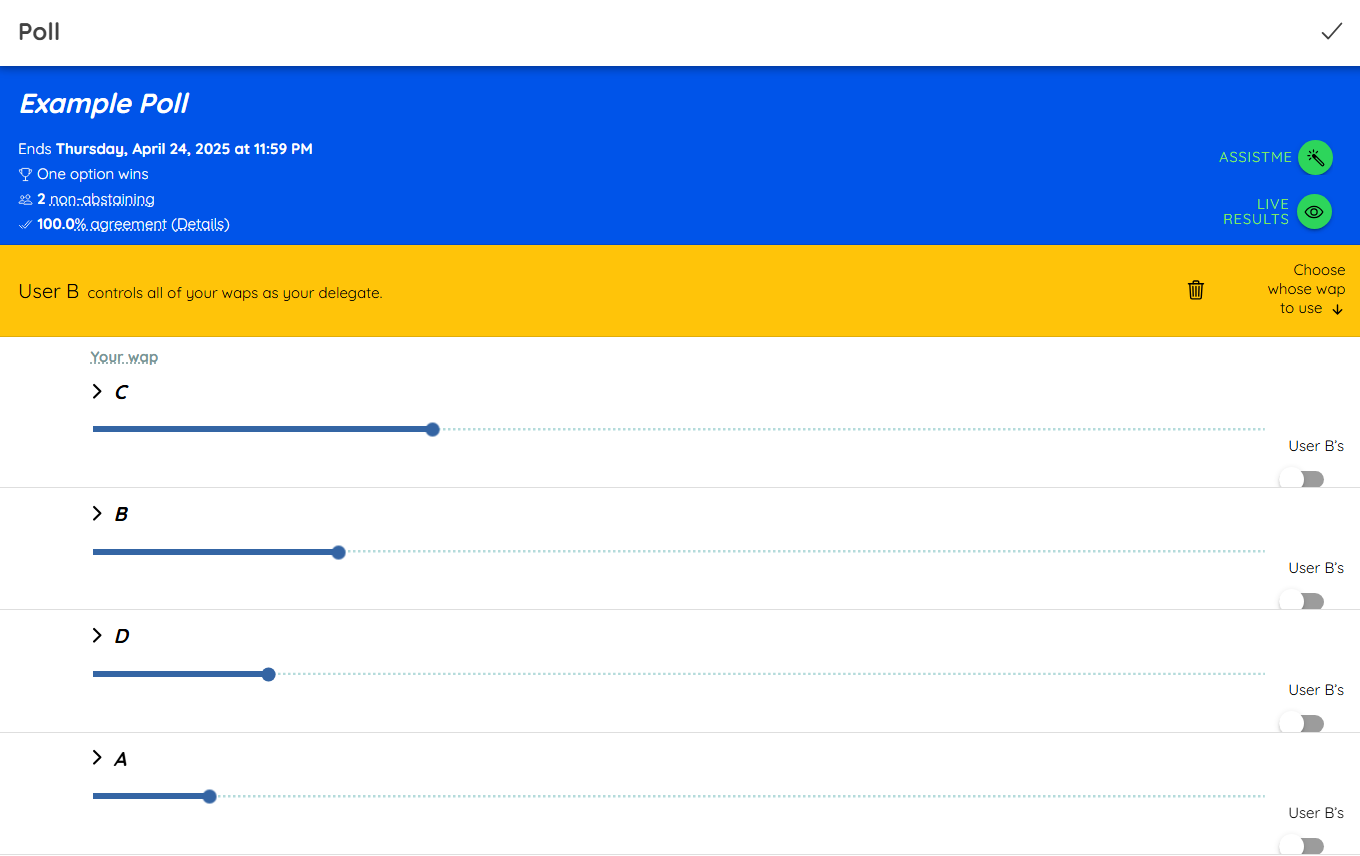
\includegraphics[width=\linewidth]{../common/vodle_screenshots/userA_after.png}
    \caption{User A (delegator) can now see that their waps are controlled by User B.}
    \label{fig:userA_after}
  \end{subfigure}

  \vspace{1em}

  \begin{subfigure}[t]{0.8\linewidth}
    \centering
    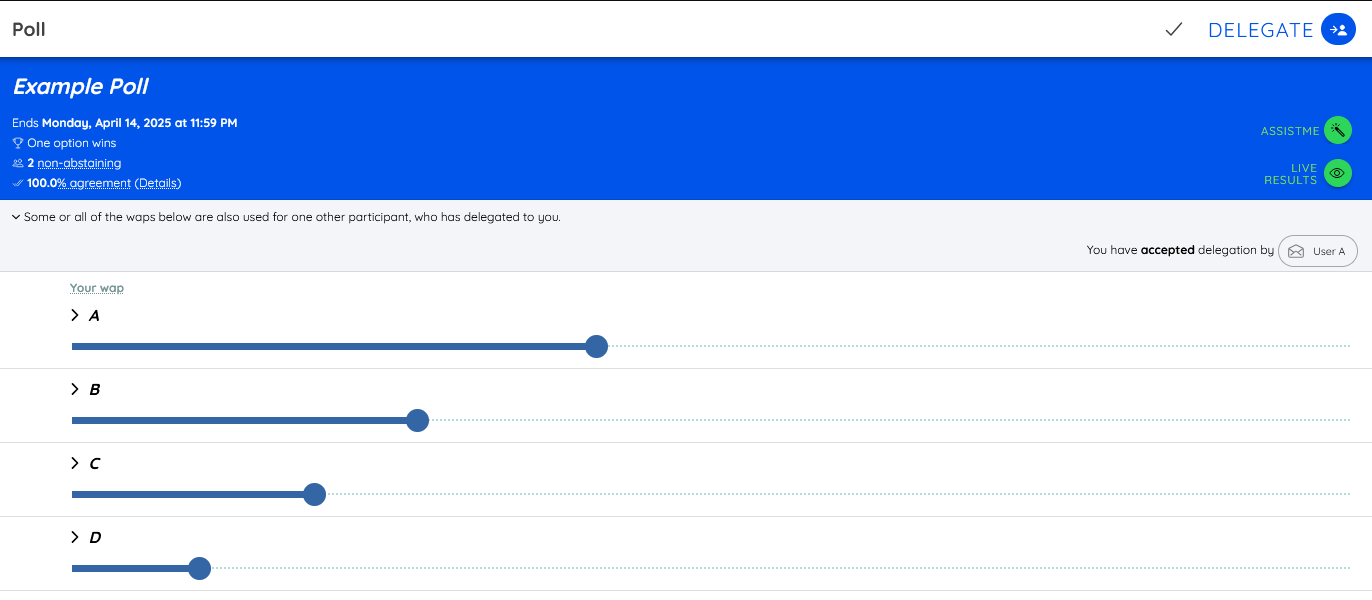
\includegraphics[width=\linewidth]{../common/initial_vodle_screenshots/userB_after.png}
    \caption{User B (delegate) can see that their vote also determines the outcome for one other user (User A).}
    \label{fig:userB_after}
  \end{subfigure}

  \caption{Delegate's (bottom) and delegator's (top) screens after a delegation has been accepted.}
  \label{fig:delegation_flow_ui}
\end{figure}
\subsection{Summary -- TODO}


\section{Implement Ranked Delegation into Vodle}\label{sec:design_ranked_delegation}
This feature introduced ranked delegation using the MinSum rule, allowing users to list fallback delegates in case their primary choice was unavailable.

\begin{itemize}
  \item UI for setting delegate rankings
  \item make sure you can't delegate the same rank twice
  \item UI for re ordering delegations
  \item New UI when making a poll to allow user to select ranked delegation.
  \item \verb|direct_delegation_map|: maps user IDs to list of ranked delegates [[delegationid, rank, status]...]
  \item Explanation and application of the MinSum rule
  \item How do we determine who is a casting voter?
  \item Implementation of ranked path resolution
  \item Illustrations and code snippets
\end{itemize}

\subsubsection{Challenges}
The MinSum rule had to be implemented efficiently using only browser-based resources. Ranking resolution had to preserve user intent while avoiding delegation ambiguity. Providing visual feedback to help users understand how rankings would resolve added an additional layer of design complexity.

\section{Implement a Vote Weighted Delegation Mechanism into Vodle}
Weighte delegation was implemented to allow users to distribute fractional influence to multiple delegates.

\begin{itemize}
  \item UI for assigning weights
  \item modify\verb|direct_delegation_map|to include weights [[delegationid, weight, status]...]
  \item Computation of weighted vote outcomes
  \item Constraints:
  \begin{itemize}
    \item Weight sum limit (\texttt{< 1.0})
    \item Error handling
  \end{itemize}
  \item Optimisations to limit database writes.
  \item Algorithm integration and frontend testing
\end{itemize}

\subsubsection{Challenges}
The weighted delegation logic needed to maintain consistency with the MaxParC aggregation model, while ensuring intuitive user experience. Edge cases (e.g., partially overlapping delegate chains or missing data) introduced complexity during testing. Rendering weight distributions clearly in the UI while keeping the interface lightweight was a recurring challenge.

\section{Implement the Ability to Delegate Individual Options to Different Users}
This feature enabled per-option delegation, allowing users to assign a different delegate for each item in a poll.

\begin{itemize}
  \item Per-option delegate selection interface
  \item Independent resolution of each delegated option
  \item talk about nested map - need to take care to serialise.
  \item \verb|direct_delegation_map|: \verb|option_id| -> \verb|user_id| -> [delegationid, null, status]
  \item \verb|inverse_indirect_map|: \verb|option_id| -> \verb|user_id| -> list of users who have delegated to them, either directly or indirectly.
  \item Storage schema modifications
\end{itemize}

\subsubsection{Challenges}
This mechanism required updates to the internal delegation logic to handle resolution at the option level. The user interface also had to be adapted to display multiple concurrent delegate selections without overwhelming the user. Debugging resolution logic for hybrid delegation modes (e.g., one direct, one split, one ranked) was non-trivial.

\section{Simulate Delegation Mechanisms -- Can Remove?}
The simulation objective was de-scoped due to time constraints and prioritisation of implementation work. While initial planning and framework selection (Mesa) were completed, no functional simulation code was delivered. The decision to drop this extension is discussed further in the Project Management chapter.

\section{Design Decisions and Trade-offs}
\begin{itemize}
  \item All logic had to run client-side due to the serverless CouchDB architecture, limiting complexity and computational resources.
  \item A consistent JSON format was required for all data models, impacting flexibility in data design.
  \item Trade-offs were made between expressive delegation types and usability, particularly in the option-specific and weighted delegation interfaces.
\end{itemize}

\section{Summary}
\begin{itemize}
  \item Each objective was successfully implemented within the constraints of the vodle platform.
  \item Challenges were primarily technical (client-side performance, real-time resolution) and design-oriented (clarity and control for users).
  \item The final implementation offers a modular, extensible delegation system that addresses the key theoretical and practical limitations outlined in earlier chapters.
\end{itemize}

